%%%%%%%%%%%%%%%%%%%%%%%%%%%%%%%%%%%%%%%%%
% The Legrand Orange Book
% LaTeX Template
% Version 2.2 (30/3/17)
%
% This template has been downloaded from:
% http://www.LaTeXTemplates.com
%
% Original author:
% Mathias Legrand (legrand.mathias@gmail.com) with modifications by:
% Vel (vel@latextemplates.com)
%
% License:
% CC BY-NC-SA 3.0 (http://creativecommons.org/licenses/by-nc-sa/3.0/)
%
% Compiling this template:
% This template uses biber for its bibliography and makeindex for its index.
% When you first open the template, compile it from the command line with the 
% commands below to make sure your LaTeX distribution is configured correctly:
%
% 1) pdflatex main
% 2) makeindex main.idx -s StyleInd.ist
% 3) biber main
% 4) pdflatex main x 2
%
% After this, when you wish to update the bibliography/index use the appropriate
% command above and make sure to compile with pdflatex several times 
% afterwards to propagate your changes to the document.
%
% This template also uses a number of packages which may need to be
% updated to the newest versions for the template to compile. It is strongly
% recommended you update your LaTeX distribution if you have any
% compilation errors.
%
% Important note:
% Chapter heading images should have a 2:1 width:height ratio,
% e.g. 920px width and 460px height.
%
%%%%%%%%%%%%%%%%%%%%%%%%%%%%%%%%%%%%%%%%%

%----------------------------------------------------------------------------------------
%	PACKAGES AND OTHER DOCUMENT CONFIGURATIONS
%----------------------------------------------------------------------------------------

\documentclass[11pt,fleqn]{book} % Default font size and left-justified equations

%----------------------------------------------------------------------------------------

%%%%%%%%%%%%%%%%%%%%%%%%%%%%%%%%%%%%%%%%%
% The Legrand Orange Book
% Structural Definitions File
% Version 2.0 (9/2/15)
%
% Original author:
% Mathias Legrand (legrand.mathias@gmail.com) with modifications by:
% Vel (vel@latextemplates.com)
% 
% This file has been downloaded from:
% http://www.LaTeXTemplates.com
%
% License:
% CC BY-NC-SA 3.0 (http://creativecommons.org/licenses/by-nc-sa/3.0/)
%
%%%%%%%%%%%%%%%%%%%%%%%%%%%%%%%%%%%%%%%%%

%----------------------------------------------------------------------------------------
%	VARIOUS REQUIRED PACKAGES AND CONFIGURATIONS
%----------------------------------------------------------------------------------------

\usepackage[top=3cm,bottom=3cm,left=3cm,right=3cm,headsep=10pt,a4paper]{geometry} % Page margins

\usepackage{graphicx} % Required for including pictures
\graphicspath{{Pictures/}} % Specifies the directory where pictures are stored

\usepackage{lipsum} % Inserts dummy text

\usepackage{tikz} % Required for drawing custom shapes

\usepackage[english]{babel} % English language/hyphenation

\usepackage{enumitem} % Customize lists
\setlist{nolistsep} % Reduce spacing between bullet points and numbered lists

\usepackage{booktabs} % Required for nicer horizontal rules in tables

\usepackage{xcolor} % Required for specifying colors by name
\definecolor{ocre}{RGB}{243,102,25} % Define the orange color used for highlighting throughout the book

%----------------------------------------------------------------------------------------
%	FONTS
%----------------------------------------------------------------------------------------

\usepackage{avant} % Use the Avantgarde font for headings
%\usepackage{times} % Use the Times font for headings
\usepackage{mathptmx} % Use the Adobe Times Roman as the default text font together with math symbols from the Sym­bol, Chancery and Com­puter Modern fonts

\usepackage{microtype} % Slightly tweak font spacing for aesthetics
\usepackage[utf8]{inputenc} % Required for including letters with accents
\usepackage[T1]{fontenc} % Use 8-bit encoding that has 256 glyphs

%----------------------------------------------------------------------------------------
%	BIBLIOGRAPHY AND INDEX
%----------------------------------------------------------------------------------------

\usepackage[style=alphabetic,citestyle=numeric,sorting=nyt,sortcites=true,autopunct=true,babel=hyphen,hyperref=true,abbreviate=false,backref=true,backend=bibtex]{biblatex}
\addbibresource{bibliography.bib} % BibTeX bibliography file
\defbibheading{bibempty}{}

\usepackage{calc} % For simpler calculation - used for spacing the index letter headings correctly
\usepackage{makeidx} % Required to make an index
\makeindex % Tells LaTeX to create the files required for indexing

%----------------------------------------------------------------------------------------
%	MAIN TABLE OF CONTENTS
%----------------------------------------------------------------------------------------

\usepackage{titletoc} % Required for manipulating the table of contents

\contentsmargin{0cm} % Removes the default margin

% Part text styling
\titlecontents{part}[0cm]
{\addvspace{20pt}\centering\large\bfseries}
{}
{}
{}

% Chapter text styling
\titlecontents{chapter}[1.25cm] % Indentation
{\addvspace{12pt}\large\sffamily\bfseries} % Spacing and font options for chapters
{\color{ocre!60}\contentslabel[\Large\thecontentslabel]{1.25cm}\color{ocre}} % Chapter number
{\color{ocre}}  
{\color{ocre!60}\normalsize\;\titlerule*[.5pc]{.}\;\thecontentspage} % Page number

% Section text styling
\titlecontents{section}[1.25cm] % Indentation
{\addvspace{3pt}\sffamily\bfseries} % Spacing and font options for sections
{\contentslabel[\thecontentslabel]{1.25cm}} % Section number
{}
{\hfill\color{black}\thecontentspage} % Page number
[]

% Subsection text styling
\titlecontents{subsection}[1.25cm] % Indentation
{\addvspace{1pt}\sffamily\small} % Spacing and font options for subsections
{\contentslabel[\thecontentslabel]{1.25cm}} % Subsection number
{}
{\ \titlerule*[.5pc]{.}\;\thecontentspage} % Page number
[]

% List of figures
\titlecontents{figure}[0em]
{\addvspace{-5pt}\sffamily}
{\thecontentslabel\hspace*{1em}}
{}
{\ \titlerule*[.5pc]{.}\;\thecontentspage}
[]

% List of tables
\titlecontents{table}[0em]
{\addvspace{-5pt}\sffamily}
{\thecontentslabel\hspace*{1em}}
{}
{\ \titlerule*[.5pc]{.}\;\thecontentspage}
[]

%----------------------------------------------------------------------------------------
%	MINI TABLE OF CONTENTS IN PART HEADS
%----------------------------------------------------------------------------------------

% Chapter text styling
\titlecontents{lchapter}[0em] % Indenting
{\addvspace{15pt}\large\sffamily\bfseries} % Spacing and font options for chapters
{\color{ocre}\contentslabel[\Large\thecontentslabel]{1.25cm}\color{ocre}} % Chapter number
{}  
{\color{ocre}\normalsize\sffamily\bfseries\;\titlerule*[.5pc]{.}\;\thecontentspage} % Page number

% Section text styling
\titlecontents{lsection}[0em] % Indenting
{\sffamily\small} % Spacing and font options for sections
{\contentslabel[\thecontentslabel]{1.25cm}} % Section number
{}
{}

% Subsection text styling
\titlecontents{lsubsection}[.5em] % Indentation
{\normalfont\footnotesize\sffamily} % Font settings
{}
{}
{}

%----------------------------------------------------------------------------------------
%	PAGE HEADERS
%----------------------------------------------------------------------------------------

\usepackage{fancyhdr} % Required for header and footer configuration

\pagestyle{fancy}
\renewcommand{\chaptermark}[1]{\markboth{\sffamily\normalsize\bfseries\chaptername\ \thechapter.\ #1}{}} % Chapter text font settings
\renewcommand{\sectionmark}[1]{\markright{\sffamily\normalsize\thesection\hspace{5pt}#1}{}} % Section text font settings
\fancyhf{} \fancyhead[LE,RO]{\sffamily\normalsize\thepage} % Font setting for the page number in the header
\fancyhead[LO]{\rightmark} % Print the nearest section name on the left side of odd pages
\fancyhead[RE]{\leftmark} % Print the current chapter name on the right side of even pages
\renewcommand{\headrulewidth}{0.5pt} % Width of the rule under the header
\addtolength{\headheight}{2.5pt} % Increase the spacing around the header slightly
\renewcommand{\footrulewidth}{0pt} % Removes the rule in the footer
\fancypagestyle{plain}{\fancyhead{}\renewcommand{\headrulewidth}{0pt}} % Style for when a plain pagestyle is specified

% Removes the header from odd empty pages at the end of chapters
\makeatletter
\renewcommand{\cleardoublepage}{
\clearpage\ifodd\c@page\else
\hbox{}
\vspace*{\fill}
\thispagestyle{empty}
\newpage
\fi}

%----------------------------------------------------------------------------------------
%	THEOREM STYLES
%----------------------------------------------------------------------------------------

\usepackage{amsmath,amsfonts,amssymb,amsthm} % For math equations, theorems, symbols, etc

\newcommand{\intoo}[2]{\mathopen{]}#1\,;#2\mathclose{[}}
\newcommand{\ud}{\mathop{\mathrm{{}d}}\mathopen{}}
\newcommand{\intff}[2]{\mathopen{[}#1\,;#2\mathclose{]}}
\newtheorem{notation}{Notation}[chapter]

% Boxed/framed environments
\newtheoremstyle{ocrenumbox}% % Theorem style name
{0pt}% Space above
{0pt}% Space below
{\normalfont}% % Body font
{}% Indent amount
{\small\bf\sffamily\color{ocre}}% % Theorem head font
{\;}% Punctuation after theorem head
{0.25em}% Space after theorem head
{\small\sffamily\color{ocre}\thmname{#1}\nobreakspace\thmnumber{\@ifnotempty{#1}{}\@upn{#2}}% Theorem text (e.g. Theorem 2.1)
\thmnote{\nobreakspace\the\thm@notefont\sffamily\bfseries\color{black}---\nobreakspace#3.}} % Optional theorem note
\renewcommand{\qedsymbol}{$\blacksquare$}% Optional qed square

\newtheoremstyle{blacknumex}% Theorem style name
{5pt}% Space above
{5pt}% Space below
{\normalfont}% Body font
{} % Indent amount
{\small\bf\sffamily}% Theorem head font
{\;}% Punctuation after theorem head
{0.25em}% Space after theorem head
{\small\sffamily{\tiny\ensuremath{\blacksquare}}\nobreakspace\thmname{#1}\nobreakspace\thmnumber{\@ifnotempty{#1}{}\@upn{#2}}% Theorem text (e.g. Theorem 2.1)
\thmnote{\nobreakspace\the\thm@notefont\sffamily\bfseries---\nobreakspace#3.}}% Optional theorem note

\newtheoremstyle{blacknumbox} % Theorem style name
{0pt}% Space above
{0pt}% Space below
{\normalfont}% Body font
{}% Indent amount
{\small\bf\sffamily}% Theorem head font
{\;}% Punctuation after theorem head
{0.25em}% Space after theorem head
{\small\sffamily\thmname{#1}\nobreakspace\thmnumber{\@ifnotempty{#1}{}\@upn{#2}}% Theorem text (e.g. Theorem 2.1)
\thmnote{\nobreakspace\the\thm@notefont\sffamily\bfseries---\nobreakspace#3.}}% Optional theorem note

% Non-boxed/non-framed environments
\newtheoremstyle{ocrenum}% % Theorem style name
{5pt}% Space above
{5pt}% Space below
{\normalfont}% % Body font
{}% Indent amount
{\small\bf\sffamily\color{ocre}}% % Theorem head font
{\;}% Punctuation after theorem head
{0.25em}% Space after theorem head
{\small\sffamily\color{ocre}\thmname{#1}\nobreakspace\thmnumber{\@ifnotempty{#1}{}\@upn{#2}}% Theorem text (e.g. Theorem 2.1)
\thmnote{\nobreakspace\the\thm@notefont\sffamily\bfseries\color{black}---\nobreakspace#3.}} % Optional theorem note
\renewcommand{\qedsymbol}{$\blacksquare$}% Optional qed square
\makeatother

% Defines the theorem text style for each type of theorem to one of the three styles above
\newcounter{dummy} 
\numberwithin{dummy}{section}
\theoremstyle{ocrenumbox}
\newtheorem{theoremeT}[dummy]{Theorem}
\newtheorem{problem}{Problem}[chapter]
\newtheorem{exerciseT}{Exercise}[chapter]
\theoremstyle{blacknumex}
\newtheorem{exampleT}{Example}[chapter]
\theoremstyle{blacknumbox}
\newtheorem{vocabulary}{Vocabulary}[chapter]
\newtheorem{definitionT}{Definition}[section]
\newtheorem{corollaryT}[dummy]{Corollary}
\theoremstyle{ocrenum}
\newtheorem{proposition}[dummy]{Proposition}

%----------------------------------------------------------------------------------------
%	DEFINITION OF COLORED BOXES
%----------------------------------------------------------------------------------------

\RequirePackage[framemethod=default]{mdframed} % Required for creating the theorem, definition, exercise and corollary boxes

% Theorem box
\newmdenv[skipabove=7pt,
skipbelow=7pt,
backgroundcolor=black!5,
linecolor=ocre,
innerleftmargin=5pt,
innerrightmargin=5pt,
innertopmargin=5pt,
leftmargin=0cm,
rightmargin=0cm,
innerbottommargin=5pt]{tBox}

% Exercise box	  
\newmdenv[skipabove=7pt,
skipbelow=7pt,
rightline=false,
leftline=true,
topline=false,
bottomline=false,
backgroundcolor=ocre!10,
linecolor=ocre,
innerleftmargin=5pt,
innerrightmargin=5pt,
innertopmargin=5pt,
innerbottommargin=5pt,
leftmargin=0cm,
rightmargin=0cm,
linewidth=4pt]{eBox}	

% Definition box
\newmdenv[skipabove=7pt,
skipbelow=7pt,
rightline=false,
leftline=true,
topline=false,
bottomline=false,
linecolor=ocre,
innerleftmargin=5pt,
innerrightmargin=5pt,
innertopmargin=0pt,
leftmargin=0cm,
rightmargin=0cm,
linewidth=4pt,
innerbottommargin=0pt]{dBox}	

% Corollary box
\newmdenv[skipabove=7pt,
skipbelow=7pt,
rightline=false,
leftline=true,
topline=false,
bottomline=false,
linecolor=gray,
backgroundcolor=black!5,
innerleftmargin=5pt,
innerrightmargin=5pt,
innertopmargin=5pt,
leftmargin=0cm,
rightmargin=0cm,
linewidth=4pt,
innerbottommargin=5pt]{cBox}

% Creates an environment for each type of theorem and assigns it a theorem text style from the "Theorem Styles" section above and a colored box from above
\newenvironment{theorem}{\begin{tBox}\begin{theoremeT}}{\end{theoremeT}\end{tBox}}
\newenvironment{exercise}{\begin{eBox}\begin{exerciseT}}{\hfill{\color{ocre}\tiny\ensuremath{\blacksquare}}\end{exerciseT}\end{eBox}}				  
\newenvironment{definition}{\begin{dBox}\begin{definitionT}}{\end{definitionT}\end{dBox}}	
\newenvironment{example}{\begin{exampleT}}{\hfill{\tiny\ensuremath{\blacksquare}}\end{exampleT}}		
\newenvironment{corollary}{\begin{cBox}\begin{corollaryT}}{\end{corollaryT}\end{cBox}}	

%----------------------------------------------------------------------------------------
%	REMARK ENVIRONMENT
%----------------------------------------------------------------------------------------

\newenvironment{remark}{\par\vspace{10pt}\small % Vertical white space above the remark and smaller font size
\begin{list}{}{
\leftmargin=35pt % Indentation on the left
\rightmargin=25pt}\item\ignorespaces % Indentation on the right
\makebox[-2.5pt]{\begin{tikzpicture}[overlay]
\node[draw=ocre!60,line width=1pt,circle,fill=ocre!25,font=\sffamily\bfseries,inner sep=2pt,outer sep=0pt] at (-15pt,0pt){\textcolor{ocre}{R}};\end{tikzpicture}} % Orange R in a circle
\advance\baselineskip -1pt}{\end{list}\vskip5pt} % Tighter line spacing and white space after remark

%----------------------------------------------------------------------------------------
%	SECTION NUMBERING IN THE MARGIN
%----------------------------------------------------------------------------------------

\makeatletter
\renewcommand{\@seccntformat}[1]{\llap{\textcolor{ocre}{\csname the#1\endcsname}\hspace{1em}}}                    
\renewcommand{\section}{\@startsection{section}{1}{\z@}
{-4ex \@plus -1ex \@minus -.4ex}
{1ex \@plus.2ex }
{\normalfont\large\sffamily\bfseries}}
\renewcommand{\subsection}{\@startsection {subsection}{2}{\z@}
{-3ex \@plus -0.1ex \@minus -.4ex}
{0.5ex \@plus.2ex }
{\normalfont\sffamily\bfseries}}
\renewcommand{\subsubsection}{\@startsection {subsubsection}{3}{\z@}
{-2ex \@plus -0.1ex \@minus -.2ex}
{.2ex \@plus.2ex }
{\normalfont\small\sffamily\bfseries}}                        
\renewcommand\paragraph{\@startsection{paragraph}{4}{\z@}
{-2ex \@plus-.2ex \@minus .2ex}
{.1ex}
{\normalfont\small\sffamily\bfseries}}

%----------------------------------------------------------------------------------------
%	PART HEADINGS
%----------------------------------------------------------------------------------------

% numbered part in the table of contents
\newcommand{\@mypartnumtocformat}[2]{%
\setlength\fboxsep{0pt}%
\noindent\colorbox{ocre!20}{\strut\parbox[c][.7cm]{\ecart}{\color{ocre!70}\Large\sffamily\bfseries\centering#1}}\hskip\esp\colorbox{ocre!40}{\strut\parbox[c][.7cm]{\linewidth-\ecart-\esp}{\Large\sffamily\centering#2}}}%
%%%%%%%%%%%%%%%%%%%%%%%%%%%%%%%%%%
% unnumbered part in the table of contents
\newcommand{\@myparttocformat}[1]{%
\setlength\fboxsep{0pt}%
\noindent\colorbox{ocre!40}{\strut\parbox[c][.7cm]{\linewidth}{\Large\sffamily\centering#1}}}%
%%%%%%%%%%%%%%%%%%%%%%%%%%%%%%%%%%
\newlength\esp
\setlength\esp{4pt}
\newlength\ecart
\setlength\ecart{1.2cm-\esp}
\newcommand{\thepartimage}{}%
\newcommand{\partimage}[1]{\renewcommand{\thepartimage}{#1}}%
\def\@part[#1]#2{%
\ifnum \c@secnumdepth >-2\relax%
\refstepcounter{part}%
\addcontentsline{toc}{part}{\texorpdfstring{\protect\@mypartnumtocformat{\thepart}{#1}}{\partname~\thepart\ ---\ #1}}
\else%
\addcontentsline{toc}{part}{\texorpdfstring{\protect\@myparttocformat{#1}}{#1}}%
\fi%
\startcontents%
\markboth{}{}%
{\thispagestyle{empty}%
\begin{tikzpicture}[remember picture,overlay]%
\node at (current page.north west){\begin{tikzpicture}[remember picture,overlay]%	
\fill[ocre!20](0cm,0cm) rectangle (\paperwidth,-\paperheight);
\node[anchor=north] at (4cm,-3.25cm){\color{ocre!40}\fontsize{220}{100}\sffamily\bfseries\thepart}; 
\node[anchor=south east] at (\paperwidth-1cm,-\paperheight+1cm){\parbox[t][][t]{8.5cm}{
\printcontents{l}{0}{\setcounter{tocdepth}{1}}%
}};
\node[anchor=north east] at (\paperwidth-1.5cm,-3.25cm){\parbox[t][][t]{15cm}{\strut\raggedleft\color{white}\fontsize{30}{30}\sffamily\bfseries#2}};
\end{tikzpicture}};
\end{tikzpicture}}%
\@endpart}
\def\@spart#1{%
\startcontents%
\phantomsection
{\thispagestyle{empty}%
\begin{tikzpicture}[remember picture,overlay]%
\node at (current page.north west){\begin{tikzpicture}[remember picture,overlay]%	
\fill[ocre!20](0cm,0cm) rectangle (\paperwidth,-\paperheight);
\node[anchor=north east] at (\paperwidth-1.5cm,-3.25cm){\parbox[t][][t]{15cm}{\strut\raggedleft\color{white}\fontsize{30}{30}\sffamily\bfseries#1}};
\end{tikzpicture}};
\end{tikzpicture}}
\addcontentsline{toc}{part}{\texorpdfstring{%
\setlength\fboxsep{0pt}%
\noindent\protect\colorbox{ocre!40}{\strut\protect\parbox[c][.7cm]{\linewidth}{\Large\sffamily\protect\centering #1\quad\mbox{}}}}{#1}}%
\@endpart}
\def\@endpart{\vfil\newpage
\if@twoside
\if@openright
\null
\thispagestyle{empty}%
\newpage
\fi
\fi
\if@tempswa
\twocolumn
\fi}

%----------------------------------------------------------------------------------------
%	CHAPTER HEADINGS
%----------------------------------------------------------------------------------------

% A switch to conditionally include a picture, implemented by  Christian Hupfer
\newif\ifusechapterimage
\usechapterimagetrue
\newcommand{\thechapterimage}{}%
\newcommand{\chapterimage}[1]{\ifusechapterimage\renewcommand{\thechapterimage}{#1}\fi}%
\newcommand{\autodot}{.}
\def\@makechapterhead#1{%
{\parindent \z@ \raggedright \normalfont
\ifnum \c@secnumdepth >\m@ne
\if@mainmatter
\begin{tikzpicture}[remember picture,overlay]
\node at (current page.north west)
{\begin{tikzpicture}[remember picture,overlay]
\node[anchor=north west,inner sep=0pt] at (0,0) {\ifusechapterimage\includegraphics[width=\paperwidth]{\thechapterimage}\fi};
\draw[anchor=west] (\Gm@lmargin,-9cm) node [line width=2pt,rounded corners=15pt,draw=ocre,fill=white,fill opacity=0.5,inner sep=15pt]{\strut\makebox[22cm]{}};
\draw[anchor=west] (\Gm@lmargin+.3cm,-9cm) node {\huge\sffamily\bfseries\color{black}\thechapter\autodot~#1\strut};
\end{tikzpicture}};
\end{tikzpicture}
\else
\begin{tikzpicture}[remember picture,overlay]
\node at (current page.north west)
{\begin{tikzpicture}[remember picture,overlay]
\node[anchor=north west,inner sep=0pt] at (0,0) {\ifusechapterimage\includegraphics[width=\paperwidth]{\thechapterimage}\fi};
\draw[anchor=west] (\Gm@lmargin,-9cm) node [line width=2pt,rounded corners=15pt,draw=ocre,fill=white,fill opacity=0.5,inner sep=15pt]{\strut\makebox[22cm]{}};
\draw[anchor=west] (\Gm@lmargin+.3cm,-9cm) node {\huge\sffamily\bfseries\color{black}#1\strut};
\end{tikzpicture}};
\end{tikzpicture}
\fi\fi\par\vspace*{270\p@}}}

%-------------------------------------------

\def\@makeschapterhead#1{%
\begin{tikzpicture}[remember picture,overlay]
\node at (current page.north west)
{\begin{tikzpicture}[remember picture,overlay]
\node[anchor=north west,inner sep=0pt] at (0,0) {\ifusechapterimage\includegraphics[width=\paperwidth]{\thechapterimage}\fi};
\draw[anchor=west] (\Gm@lmargin,-9cm) node [line width=2pt,rounded corners=15pt,draw=ocre,fill=white,fill opacity=0.5,inner sep=15pt]{\strut\makebox[22cm]{}};
\draw[anchor=west] (\Gm@lmargin+.3cm,-9cm) node {\huge\sffamily\bfseries\color{black}#1\strut};
\end{tikzpicture}};
\end{tikzpicture}
\par\vspace*{270\p@}}
\makeatother

%----------------------------------------------------------------------------------------
%	HYPERLINKS IN THE DOCUMENTS
%----------------------------------------------------------------------------------------

\usepackage{hyperref}
\hypersetup{hidelinks,backref=true,pagebackref=true,hyperindex=true,colorlinks=false,breaklinks=true,urlcolor= ocre,bookmarks=true,bookmarksopen=false,pdftitle={Title},pdfauthor={Author}}
\usepackage{bookmark}
\bookmarksetup{
open,
numbered,
addtohook={%
\ifnum\bookmarkget{level}=0 % chapter
\bookmarksetup{bold}%
\fi
\ifnum\bookmarkget{level}=-1 % part
\bookmarksetup{color=ocre,bold}%
\fi
}
}
 % Insert the commands.tex file which contains the majority of the structure behind the template

\begin{document}

%----------------------------------------------------------------------------------------
%	TITLE PAGE
%----------------------------------------------------------------------------------------

\begingroup
\thispagestyle{empty}
\begin{tikzpicture}[remember picture,overlay]
\node[inner sep=0pt] (background) at (current page.center) {
\includegraphics[width=\paperwidth]{background}};
\draw (current page.center) node [fill=ocre!30!white,fill opacity=0.6,text opacity=1,inner sep=1cm]{\Huge\centering\bfseries\sffamily\parbox[c][][t]{\paperwidth}{\centering The Search for a Title\\[15pt] % Book title
{\Large A Profound Subtitle}\\[20pt] % Subtitle
{\huge Dr. John Smith}}}; % Author name
\end{tikzpicture}
\vfill
\endgroup

%----------------------------------------------------------------------------------------
%	COPYRIGHT PAGE
%----------------------------------------------------------------------------------------

\newpage
~\vfill
\thispagestyle{empty}

\noindent Copyright \copyright\ 2013 John Smith\\ % Copyright notice

\noindent \textsc{Published by Publisher}\\ % Publisher

\noindent \textsc{book-website.com}\\ % URL

\noindent Licensed under the Creative Commons Attribution-NonCommercial 3.0 Unported License (the ``License''). You may not use this file except in compliance with the License. You may obtain a copy of the License at \url{http://creativecommons.org/licenses/by-nc/3.0}. Unless required by applicable law or agreed to in writing, software distributed under the License is distributed on an \textsc{``as is'' basis, without warranties or conditions of any kind}, either express or implied. See the License for the specific language governing permissions and limitations under the License.\\ % License information

\noindent \textit{First printing, March 2013} % Printing/edition date

%----------------------------------------------------------------------------------------
%	TABLE OF CONTENTS
%----------------------------------------------------------------------------------------

%\usechapterimagefalse % If you don't want to include a chapter image, use this to toggle images off - it can be enabled later with \usechapterimagetrue

\chapterimage{chapter_head_1.pdf} % Table of contents heading image

\pagestyle{empty} % No headers

\tableofcontents % Print the table of contents itself

\cleardoublepage % Forces the first chapter to start on an odd page so it's on the right

\pagestyle{fancy} % Print headers again

%----------------------------------------------------------------------------------------
%	PART
%----------------------------------------------------------------------------------------

\part{Part One}

%----------------------------------------------------------------------------------------
%	CHAPTER 1
%----------------------------------------------------------------------------------------

\chapterimage{chapter_head_2.pdf} % Chapter heading image

\chapter{Logika Matematika}

\section{Pernyataan Berkuantor}\index{Pernyataan Berkuantor}

Kuantor dari suatu pernyataan adalah istilah yang digunakan untuk menyatakan “berapa banyak” objek di dalam suatu kalimat atau pembicaraan. Selain untuk menyatakan kuantifikasi, kuantor juga biasa digunakan untuk mengubah kalimat terbuka menjadi suatu kalimat deklaratif.

Definisi : Suatu fungsi pernyataan adalah suatu kalimat terbuka di dalam semesta pembicaraan (semesta pembicaraan diberikan secara eksplisit atau implisit).
Perhatikan dua pernyataan berikut:
1.    Semua planet dalam sistem tata surya mengelilingi matahari.
2.    Ada ikan di laut yang menyusui.
Pernyataan yang mengandung kata semua atau setiap seperti pada pernyataan (1) disebut pernyataan berkuantor universal (kuantor umum). Ungkapan untuk semua atau untuk setiap, disebut kuantor universal atau kuantor umum. Sedangkan pernyataan yang mengandung kata ada atau beberapa seperti pada pernyataan (2) disebut pernyataan berkuantor eksistensial (kuantor khusus). Ungkapan beberapa atau ada disebut kuantor eksistensial atau kuantor khusus.

%------------------------------------------------

\section{Pernyataan Penyangkal (Lingkaran)}\index{Pernyataan Penyangkal  (Lingkaran)}

Dari sebuah pernyataan tunggal (atau majemuk), kita bisa membuat sebuah pernyataan baru berupa “ingkaran” dari pernyataan itu. “ingkaran” disebut juga “negasi” atau “penyangkalan”. Ingkaran menggunakan operasi uner (monar) “” atau “”.

Jika suatu pernyataan p benar, maka negasinya p salah, dan jika sebaliknya pernyataan p salah, maka negasinya p benar.

Perhatikan cara membuat ingkaran dari sebuah pernyataan serta menentukan nilai kebenarannya!

1. p         : kayu memuai bila dipanaskan (S)

~ p      : kayu tidak memuai bila dipanaskan (B)

2.  r          : 3 bilangan positif (B)

~ r        : (cara mengingkar seperti ini salah)

3 bilangan negative

(Seharusnya) 3 bukan bilangan positif  (S)

Nilai kebenaran

Jika p suatu pernyataan benilai benar, maka  ~p bernilai salah dan sebaliknya jika p bernilai salah maka ~p bernilai benar

Konjungsi 

Gabungan  dua  pernyataan  tunggal  yang  menggunakan  kata penghubung  “dan”  sehingga  terbentuk  pernyataan majemuk  disebut konjungsi. Konjungsi mempunyai kemiripan dengan operasi irisan () pada  himpunan.  Sehingga  sifat-sifat  irisan  dapat  digunakan  untuk mempelajari  bagian  ini.



%------------------------------------------------

\section{Penarikan Kesimpulan}\index{Penarikan Kesimpulan}

Lists are useful to present information in a concise and/or ordered way\footnote{Footnote example...}.

\subsection{Numbered List}\index{Lists!Numbered List}

\begin{enumerate}
\item The first item
\item The second item
\item The third item
\end{enumerate}

\subsection{Bullet Points}\index{Lists!Bullet Points}

\begin{itemize}
\item The first item
\item The second item
\item The third item
\end{itemize}

\subsection{Descriptions and Definitions}\index{Lists!Descriptions and Definitions}

\begin{description}
\item[Name] Description
\item[Word] Definition
\item[Comment] Elaboration
\end{description}

%----------------------------------------------------------------------------------------
%	CHAPTER 2
%----------------------------------------------------------------------------------------

\chapter{Induksi Matematika}

\section{Metode Pembuktian Langsung dan Tidak Langsung}\index{Metode Pembuktian Langsung dan Tidak Langsung}

This is an example of theorems.

\subsection{Several equations}\index{Theorems!Several Equations}
This is a theorem consisting of several equations.

\begin{theorem}[Name of the theorem]
In $E=\mathbb{R}^n$ all norms are equivalent. It has the properties:
\begin{align}
& \big| ||\mathbf{x}|| - ||\mathbf{y}|| \big|\leq || \mathbf{x}- \mathbf{y}||\\
&  ||\sum_{i=1}^n\mathbf{x}_i||\leq \sum_{i=1}^n||\mathbf{x}_i||\quad\text{where $n$ is a finite integer}
\end{align}
\end{theorem}

\subsection{Single Line}\index{Theorems!Single Line}
This is a theorem consisting of just one line.

\begin{theorem}
A set $\mathcal{D}(G)$ in dense in $L^2(G)$, $|\cdot|_0$. 
\end{theorem}

%------------------------------------------------

\section{Kontradiksi}\index{Kontradiksi}

This is an example of a definition. A definition could be mathematical or it could define a concept.

\begin{definition}[Definition name]
Given a vector space $E$, a norm on $E$ is an application, denoted $||\cdot||$, $E$ in $\mathbb{R}^+=[0,+\infty[$ such that:
\begin{align}
& ||\mathbf{x}||=0\ \Rightarrow\ \mathbf{x}=\mathbf{0}\\
& ||\lambda \mathbf{x}||=|\lambda|\cdot ||\mathbf{x}||\\
& ||\mathbf{x}+\mathbf{y}||\leq ||\mathbf{x}||+||\mathbf{y}||
\end{align}
\end{definition}

%------------------------------------------------

\section{Induksi Matematis}\index{Induksi Matematis}

\begin{notation}
Given an open subset $G$ of $\mathbb{R}^n$, the set of functions $\varphi$ are:
\begin{enumerate}
\item Bounded support $G$;
\item Infinitely differentiable;
\end{enumerate}
a vector space is denoted by $\mathcal{D}(G)$. 
\end{notation}

%------------------------------------------------

\section{Remarks}\index{Remarks}

This is an example of a remark.

\begin{remark}
The concepts presented here are now in conventional employment in mathematics. Vector spaces are taken over the field $\mathbb{K}=\mathbb{R}$, however, established properties are easily extended to $\mathbb{K}=\mathbb{C}$.
\end{remark}

%------------------------------------------------

\section{Corollaries}\index{Corollaries}

This is an example of a corollary.

\begin{corollary}[Corollary name]
The concepts presented here are now in conventional employment in mathematics. Vector spaces are taken over the field $\mathbb{K}=\mathbb{R}$, however, established properties are easily extended to $\mathbb{K}=\mathbb{C}$.
\end{corollary}

%------------------------------------------------

\section{Kontradiksi}\index{Kontradiksi}

This is an example of propositions.

\subsection{Several equations}\index{Propositions!Several Equations}

\begin{proposition}[Proposition name]
It has the properties:
\begin{align}
& \big| ||\mathbf{x}|| - ||\mathbf{y}|| \big|\leq || \mathbf{x}- \mathbf{y}||\\
&  ||\sum_{i=1}^n\mathbf{x}_i||\leq \sum_{i=1}^n||\mathbf{x}_i||\quad\text{where $n$ is a finite integer}
\end{align}
\end{proposition}

\subsection{Single Line}\index{Propositions!Single Line}

\begin{proposition} 
Let $f,g\in L^2(G)$; if $\forall \varphi\in\mathcal{D}(G)$, $(f,\varphi)_0=(g,\varphi)_0$ then $f = g$. 
\end{proposition}

%------------------------------------------------

\section{Examples}\index{Examples}

This is an example of examples.

\subsection{Equation and Text}\index{Examples!Equation and Text}

\begin{example}
Let $G=\{x\in\mathbb{R}^2:|x|<3\}$ and denoted by: $x^0=(1,1)$; consider the function:
\begin{equation}
f(x)=\left\{\begin{aligned} & \mathrm{e}^{|x|} & & \text{si $|x-x^0|\leq 1/2$}\\
& 0 & & \text{si $|x-x^0|> 1/2$}\end{aligned}\right.
\end{equation}
The function $f$ has bounded support, we can take $A=\{x\in\mathbb{R}^2:|x-x^0|\leq 1/2+\epsilon\}$ for all $\epsilon\in\intoo{0}{5/2-\sqrt{2}}$.
\end{example}

\subsection{Paragraph of Text}\index{Examples!Paragraph of Text}

\begin{example}[Example name]
\lipsum[2]
\end{example}

%------------------------------------------------

\section{Exercises}\index{Exercises}

This is an example of an exercise.

\begin{exercise}
This is a good place to ask a question to test learning progress or further cement ideas into students' minds.
\end{exercise}

%------------------------------------------------

\section{Problems}\index{Problems}

\begin{problem}
What is the average airspeed velocity of an unladen swallow?
\end{problem}

%------------------------------------------------

\section{Vocabulary}\index{Vocabulary}

Define a word to improve a students' vocabulary.

\begin{vocabulary}[Word]
Definition of word.
\end{vocabulary}
%----------------------------------------------------------------------------------------
%	CHAPTER 3
%----------------------------------------------------------------------------------------

\chapterimage{chapter_head_2.pdf} % Chapter heading image

\chapter{Pertidaksamaan Linear Dua Variabel}

\section{Pengertian Pertidaksamaan Linear Dua Variabel}\index{Pengertian Pertidaksamaan Linear Dua Variabel}

\section{Penerapan Pertidaksamaan Linear Dua Variabel}\index{Penerapan Pertidaksamaan Linear Dua Variabel}

%----------------------------------------------------------------------------------------
%	CHAPTER 4
%----------------------------------------------------------------------------------------

\chapterimage{chapter_head_2.pdf} % Chapter heading image

\chapter{Program Linear Dua Variabel}

\section{Pengertian Program Linear Dua Variabel}\index{Pengertian Program Linear Dua Variabel}

\section{Sistem Pertidaksamaan Linear Dua Variabel}\index{Sistem Pertidaksamaan Linear Dua Variabel}

\section{Nilai Optimum Fungsi Objektif}\index{Nilai Optimum Fungsi Objektif}

\section{Penerapan Program Linier Dua Variabel}\index{Penerapan Program Linier Dua Variabel}

%----------------------------------------------------------------------------------------
%	CHAPTER 5
%----------------------------------------------------------------------------------------

\chapterimage{chapter_head_2.pdf} % Chapter heading image

\chapter{Matriks}

\section{Pengertian Matriks}\index{Pengertian Matriks}

\section{Operasi Matriks}\index{Operasi Matriks}

\section{Determinan dan Invers Matriks Berorde 2x2 dan 3x3 }\index{Determinan dan Invers Matriks Berorde 2x2 dan 3x3 }

\section{Pemakaian Matriks Pada Pransformasi Geometri}\index{Pemakaian Matriks Pada Pransformasi Geometri}

%----------------------------------------------------------------------------------------
%	CHAPTER 6
%----------------------------------------------------------------------------------------

\chapterimage{chapter_head_2.pdf} % Chapter heading image

\chapter{Barisan dan Deret}

\section{Pola Bilangan}\index{Pola Bilangan}

\section{Barisan dan Deret Aritmatika}\index{Barisan dan Deret Aritmatika}
Pengertian Barisan Aritmatika
Sebelum memahami pengertian barisan aritmatika kita harus mengetahui terlebih dahulumengenai pengertian basiran bilangan. Barisan bilangan merupakan sebuah urutan dari bilangan yang dibentuk dengan berdasarkan kepada aturan-aturan tertentu. Edangkan barisan aritmetika dapat didefinisikan sebagai suatu barisan bilangan yang tiap-tiap pasangan suku yang berurutan mengandung nilai selisih yang sama persis, contohnya adalah barisan bilangan: 2, 4 , 6, 8, 10, 12, 14, …

Barisan bilangan tersebut dapat disebut sebagai barisana aritmatika karena masing-masing suku memiliki selisih yang sama yaitu 2. Nilai selisih yang muncul pada barisan aritmatika biasa dilambangkan dengan menggunakan huruf b. Setiap bilangan yang membentuk urutan suatu barisan aritmatika disebut dengan suku. Suku ke n dari sebuah barisan aritmatika dapat disimbolkan dengan lambang Un jadi untuk menuliskan suku ke 3 dari sebuah barisan kita dapat menulis U3. Namun, ada pengecualian khusus untuk suku pertama di dalam sebuah barisan bilangan, suku pertama disimbolkan dengan menggunakan huruf a.

Maka, secara umum suatu barian aritmatika memiliki bentuk :

U1,U2,U3,U4,U5,…Un-1
a, atb, a+2b, a+3b, a+4b,…a+(n-1)b

Cara Menentukan Rumus suku ke-n dari Sebuah Barisan
Pada barisan aritmatika, mencaru rumus suku ke-n menjadi lebih mudah karena memiliki nilai selisih yang sama, sehingga rumusnya adalah:

U2 = a + b
U3 = u2 + b = (a + b) + b = a + 2b
U4 = u3 + b = (a + 2b) + b = a + 3b
U5 = u4 + b = (a + 3b) + b = a + 4b
U6 = u5 + b = (a + 4b) + b = a + 5b
U7 = u6 + b = (a + 5b) + b = a + 6b
.
\section{Barisan dan Deret Geometri}\index{Barisan dan Deret Geometri}

%----------------------------------------------------------------------------------------
%	PART
%----------------------------------------------------------------------------------------

\part{Part Two}

%----------------------------------------------------------------------------------------
%	CHAPTER 7
%----------------------------------------------------------------------------------------

\chapterimage{chapter_head_1.pdf} % Chapter heading image

\chapter{Limit Fungsi Aljabar}

\section{Table}\index{Table}

\begin{table}[h]
\centering
\begin{tabular}{l l l}
\toprule
\textbf{Treatments} & \textbf{Response 1} & \textbf{Response 2}\\
\midrule
Treatment 1 & 0.0003262 & 0.562 \\
Treatment 2 & 0.0015681 & 0.910 \\
Treatment 3 & 0.0009271 & 0.296 \\
\bottomrule
\end{tabular}
\caption{Table caption}
\end{table}

%------------------------------------------------

\section{Figure}\index{Figure}

\begin{figure}[h]
\centering
\includegraphics[scale=0.5]{placeholder}
\caption{Figure caption}
\end{figure}

%----------------------------------------------------------------------------------------
%	CHAPTER 8
%----------------------------------------------------------------------------------------

\chapterimage{chapter_head_2.pdf} % Chapter heading image

\chapter{Turunan Fungsi Aljabar}

\section{Pengertian Turunan}\index{Pengertian Turunan}

\section{Sifat-Sifat Turunan Fungsi Aljabar}\index{Sifat-Sifat Turunan Fungsi Aljabar}

\section{Penerapan Turunan Fungsi Aljabar}\index{Penerapan Turunan Fungsi Aljabar}

\section{Nilai-Nilai Stasioner}\index{Nilai-Nilai Stasioner}

\section{Aplikasi Turunan}\index{Aplikasi Turunan}
Konsep turunan adalah subjek yang banyak berperan dalam aplikasi matematika di kehidupan sehari-hari di berbagai bidang. Konsep turunan digunakan untuk
menentukan interval fungsi naik/turun, keoptimalan fungsi dan titik belok suatu kurva.
\subsection{Fungsi Naik dan Fungsi Turun}
Coba bayangkan ketika kamu pergi ke plaza atau mall, di sana kita temukan ekskalator atau lift. Gerakan lift dan ekskalator saat naik dapat diilustrasikan sebagai fungsi naik. Demikian juga gerakan lift dan ekskalator saat turun dapat diilustrasikan sebagai fungsi turun. Amatilah beberapa grafik fungsi naik dan turun di bawah ini dan coba tuliskan cirri-ciri fungsi naik dan fungsi turun sebagai ide untuk mendefinisikan fungsi naik dan turun.

Beberapa grafik fungsi turun dari kiri ke kanan

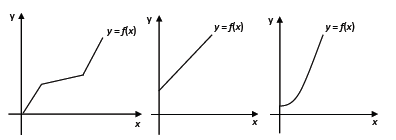
\includegraphics[width=6cm,height=3cm]{naikturun1.png}

Beberapa grafik fungsi naik dari kiri ke kanan

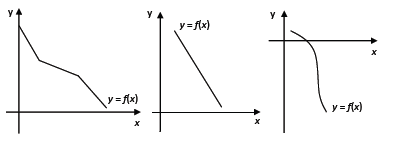
\includegraphics[width=6cm,height=3cm]{naikturun2.png}

Dari beberapa contoh grafik fungsi naik dan turun di atas,mari kita definisikan fungsi naik dan turun sebagai berikut.

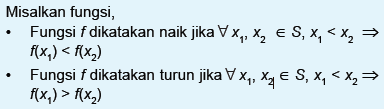
\includegraphics[width=10cm,height=3cm]{naikturun3.png}

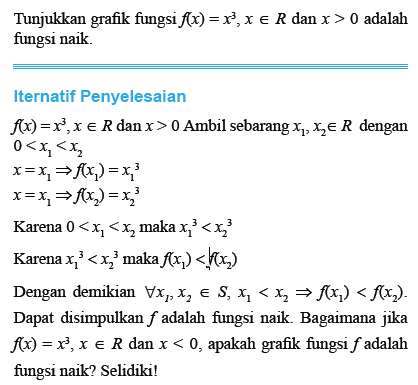
\includegraphics[width=10cm,height=7cm]{naikturun4.png}

\subsection{Aplikasi Turunan dalam Permasalahan Fungsi Naik dan Fungsi Turun}

Mari kita bahas aplikasi turunan dalam permasalahan fungsi naik dan fungsi turun dengan memperhatikan dan mengamati permasalahan berikut.\\

\textbf{Masalah 1}

Seorang nelayan melihat seekor lumba-lumba sedang berenang mengikuti kecepatan perahu mereka. Lumba-lumba tersebut berenang cepat, terkadang menyelam dan tiba-tiba melayang ke permukakaan air laut. Pada saat nelayan tersebut melihat lumba-lumba menyelam maka ia akan melihatnya melayang ke permukaan 15 detik kemudian dan kembali ke permukaan air laut setelah 3 detik di udara. Demikan pergerakan lumba-lumba tersebut diamati berperiode dalam beberapa interval waktu pengamatan.

Dari ilustrasi diatas, dapatkah kamu sketsa pergerakan lumba-lumba tersebut dalam 2 periode? Ingat pengertian periode pada pelajaran trigonometri di kelas X. Dapatkah kamu tentukan pada interval waktu berapakah lumbalumba tersebut bergerak naik atau turun? Dapatkah kamu temukan konsep fungsi naik/turun?\\

\textbf{Alternatif Penyelesaian:}

Sketsa pergerakan lumba-lumba dalam pengamatan tertentu

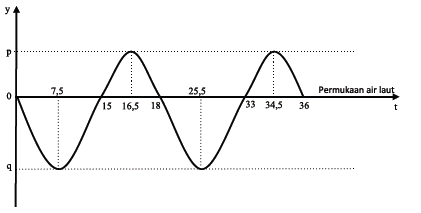
\includegraphics[width=12cm,height=5cm]{naikturun5.png}

Sketsa pergerakan naik/turun lumba-lumba dalam pengamatan tertentu

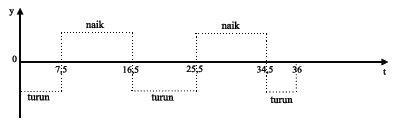
\includegraphics[width=12cm,height=5cm]{naikturun6.png}

Secara geometri pada sketsa di atas, lumba-lumba bergerak turun di interval 0 < t < 7,5 atau 16,5 < t < 25,5 atau 34,5 < t < 36 dan disebut bergerak naik di interval 7,5 < t < 16,5 atau 25,5 < t < 34,5.
%-------------Sesi 2---------------------------------
Coba kamu amati beberapa garis singgung yang menyinggung kurva di saat fungsi naik atau turun di bawah ini. Garis singgung 1 dan 3 menyinggung kurva pada saat fungsi naik dan garis singgung 2 dan 4 menyinggung kurva pada saat fungsi turun.

Garis singgung di interval fungsi naik/turun

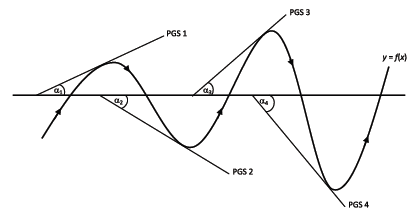
\includegraphics[width=14cm,height=7cm]{naikturun7.png}

Selanjutnya, mari kita bahas hubungan persamaan garis singgung dengan fungsi naik atau turun. Pada konsep
persamaan garis lurus, gradien garis adalah tangen sudut yang dibentuk oleh garis itu sendiri dengan sumbu x positif.Pada persamaan garis singgung, gradien adalah tangen sudut garis tersebut dengan sumbu positif sama dengan nilai turunan pertama di titik singgungnya. Pada gambar di atas, misalkan besar masing-masing sudut adalah 0 < $\propto $1 < 900 < $\propto $2 < 900 < $\propto $3 < 900 < $\propto $4 < 900 sehingga nilai
gradien atau tangen sudut setiap garis singgung ditunjukkan pada tabel berikut:

\begin{center}
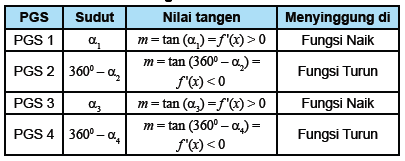
\includegraphics{naikturun8.png}
\end{center}

Coba kamu amati Gambar diatas dan Tabel sebelumnya Apakah kamu melihat konsep fungsi naik/turun. Coba kamu perhatikan kesimpulan berikut:

Jika garis singgung menyinggung di grafik fungsi naik maka garis singgung akan membentuk 

sudut terhadap sumbu x positif di kuadran I. Hal ini menyebabkan besar gradien adalah positif 

atau m = f '(x) > 0.

Jika garis singgung menyinggung di grafik fungsi turunmaka garis singgung akan membentuk 

sudut terhadap sumbu x positif di kuadran IV. Hal ini menyebabkan besar gradien adalah negatif 

atau m = f '(x) < 0.

Dengan demikian, dapat kita simpulkan bahwa fungsi f(x) yang dapat diturunkan pada interval I, akan mempunyai kondisi sebagai berikut:

\begin{center}
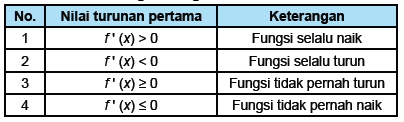
\includegraphics{naikturun9.png}
\end{center}

Misalkan f adalah fungsi bernilai real dan dapat
diturunkan pada setiap x $\in $I maka

1. Jika f '(x) > 0 maka fungsi selalu naik pada interval I.

2. Jika f '(x) < 0 maka fungsi selalu turun pada interval I.

3. Jika f '(x) $\geqslant $0 maka fungsi tidak pernah turun pada interval I.

4. Jika f '(x) $\leqslant $0 maka fungsi tidak pernah naik pada interval I.

Konsep di atas dapat digunakan jika kita sudah memiliki fungsi yang akan dianalisis. Tetapi banyak kasus seharihari harus dimodelkan terlebih dahulu sebelum dianalisis. Perhatikan kembali permasalahan berikut!\\

\textbf{Masalah:}

Tiga orang anak sedang berlomba melempar buah mangga di ketinggian 10 meter. Mereka berbaris menghadap pohon mangga sejauh 5 meter. Anak pertama akan melempar buah mangga tersebut kemudian akan dilanjutkan dengan anak kedua bila tidak mengenai sasaran. Lintasan lemparan setiap anak membentuk kurva parabola. Lemparan anak pertama mencapai ketinggian 9 meter dan batu jatuh 12 meter dari mereka. Lemparan anak kedua melintas di atas sasaran setinggi 5 meter. Anak ketiga berhasil mengenai sasaran. Tentu saja pemenangnya anak ketiga, bukan?
\\

\textbf{Permasalahan!}

Dapatkah kamu mensketsa lintasan lemparan ketiga anak tersebut? Dapatkah kamu membuat model matematika lintasan lemparan? Dapatkah kamu menentukan interval jarak agar masing-masing lemparan naik atau turun berdasarkan konsep turunan?\\


\textbf{Alternatif Penyelesaian}

\textbf{a. Sketsa Lintasan Lemparan}

Permasalahan di atas dapat kita analisis setelah kita modelkan fungsinya. Misalkan posisi awal mereka melempar adalah posisi titik asal O(0,0) pada koordinat kartesius, sehingga sketsa permasalahan di atas adalah sebagai berikut.

\begin{center}
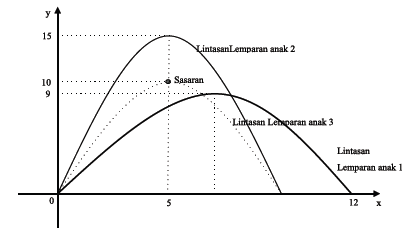
\includegraphics{naikturun10.png}
\end{center}

\textbf{b. Model Lintasan Lemparan}

Kamu masih ingat konsep fungsi kuadrat, bukan? Ingat
kembali konsep fungsi kuadrat yang melalui titik puncak
P($x_{p}, y_{p}) $dan titik sembarang P(x, y) adalah y – $y_{p} = a(x
$– $x_{p})^2 $sementara fungsi kuadrat yang melalui akar-akar x1,
x2 dan titik sembarang P(x, y) adalah y = a(x – $x_{1})(x $– $x_{2}),
$dengan $x_{p}= \dfrac{x_{1}-x_{2}}{2}
$dan a $\neq $0, a bilangan real. Jadi, model
lintasan lemparan setiap anak tersebut adalah:

\textbf{Lintasan lemparan anak pertama}

Lintasan melalui titik O(0,0) dan puncak $p_{1}$(6,9).

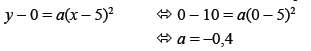
\includegraphics{naikturun11.png}

Fungsi lintasan lemparan anak pertama adalah y = –0,25$x^{2} $+ 3x.\\

\textbf{Lintasan lemparan anak kedua}

Lintasan melalui titik O(0,0) dan puncak $P_{2}$(5,15).

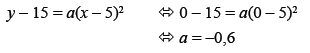
\includegraphics{naikturun12.png}

Fungsi lintasan lemparan anak kedua adalah y = –0,6$x^{2} $+ 6x.\\

\textbf{Lintasan lemparan anak ketiga}

Lintasan melalui titik O(0,0) dan puncak P3(5,10).

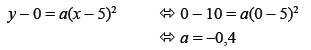
\includegraphics{naikturun13.png}

Fungsi lintasan lemparan anak ketiga adalah y = –0,4x2 +
4x.

\section{Persamaan Garis Singgung dan Garis Normal}\index{Persamaan Garis Singgung dan Garis Normal}
%----------------------------------------------------------------------------------------
%	CHAPTER 9
%----------------------------------------------------------------------------------------

\chapterimage{chapter_head_2.pdf} % Chapter heading image

\chapter{Integral Tak Tentu Fungsi Aljabar}

\section{Pengertian Integral Tak Tentu Fungsi Aljabar}\index{Pengertian Integral Tak Tentu Fungsi Aljabar}

\section{Sifat-Sifat Integral Tak Tentu Fungsi Aljabar}\index{Sifat-Sifat Integral Tak Tentu Fungsi Aljabar}

\section{Penerapan Integral Tak Tentu Fungsi Aljabar}\index{Penerapan Integral Tak Tentu Fungsi Aljabar}


%----------------------------------------------------------------------------------------

%	BIBLIOGRAPHY
%----------------------------------------------------------------------------------------

\chapter*{Bibliography}
\addcontentsline{toc}{chapter}{\textcolor{ocre}{Bibliography}}
\section*{Books}
\addcontentsline{toc}{section}{Books}
\printbibliography[heading=bibempty,type=book]
\section*{Articles}
\addcontentsline{toc}{section}{Articles}
\printbibliography[heading=bibempty,type=article]

%----------------------------------------------------------------------------------------
%	INDEX
%----------------------------------------------------------------------------------------

\cleardoublepage
\phantomsection
\setlength{\columnsep}{0.75cm}
\addcontentsline{toc}{chapter}{\textcolor{ocre}{Index}}
\printindex

%----------------------------------------------------------------------------------------

\end{document}
